\documentclass{article}

\usepackage[normalem]{ulem}
\usepackage{fancyhdr}
\usepackage[parfill]{parskip}
\usepackage{tikz}
\usepackage{pgfplots}
\usepackage{multicol}
\usepackage[version=3]{mhchem}
\usepackage{SIunits}

\pagestyle{fancyplain}

\pgfplotsset{compat=1.7}

\title{Electromagnetic induction}
\author{Todd Davies}
\date{\today}

\begin{document}

\rhead{Electromagnetic induction}
\lhead{\today}

\maketitle

\section*{Equations to learn}
\thispagestyle{empty}

\begin{itemize}

	\item The magentic field of magnetic flux density $B$ passing through an
	area $A$ is equal to:

	\[
		\phi = BAcos\theta
	\]

	\item The magnetic flux linking a coil of $N$ turns is the magnetic flux
	linkage.

	\[
		\textrm{\it Magnetic flux linkage} = N\phi
	\]
	
	\item Faraday's law states that the magentude of the induced e.m.f is equal
	to the rate of change of magnetic flux linkage:

	\[
		E = \frac{\Delta(N\phi)}{\Delta t} = 
			\frac{\Delta(BANcos\theta)}{\Delta t}
	\]

	\item The equation relating the voltage and number of turns in the coils of
	a transformer is:

	\[
		\frac{V_s}{V_p} = \frac{n_s}{n_p}
	\]

	If the transformer is 100\% efficient, then:

	\[
		V_pI_p = V_sI_s
	\]

\end{itemize}

\section*{Generating electricity}

Electricity can be generated by moving an electrical conductor inside a magnetic
field to generate an electromotive force. The magnitude of the current induced
in the wire depends on:

\begin{itemize}

	\item The magnitude of the magnetic flux density.

	\item The length of the wire in the field.

	\item The speed of movement of the wire.

\end{itemize}

If the wire is shaped into a coil:

\begin{itemize}

	\item The magnitude of the magnetic flux density.

	\item The cross sectional area of the coil.

	\item The number of turns of wire.

	\item The rate at which the coil turns in the field.

\end{itemize}

\section*{How is an e.m.f. generated?}

When a conductor moves around inside a magnetic field, it generates electricity.
This happens since the conductor {\it cuts} through magnetic field lines as it
moves in the magnetic field.

{\it N.b. it doesn't matter whether the magnetic field moves or the conductor
moves; the result is the same, magnetic field lines are crossed and there will
be an induced current.}

\subsection*{Coils of wire}

The effect of electromagnetic induction is multiplied by $N$ times if we use a
coil of wire with $N$ turns instead of a single wire.

\subsection*{Direction of current}

We can use Fleming's right hand dynamo rule in order to predict the direction of
current flow.

\begin{center}
	\includegraphics[scale=0.6]{fleming_right_hand_dynamo_rule}
\end{center}

If the conductor is not part of a complete electrical circuit, then an e.m.f.
will still be generated. However, charge will just accumulate at opposite ends
of the conductor.

\subsection*{Magnetic flux and linkage}

Remember how the magnetic flux density is defined by $B = \frac{F}{IL}$, well
now we can find the magnetic flux ($\phi$) per unit area using the following
equation:

\[
	\phi = BA
\]

This equation requires that $B$ is perpendicular to the area $A$. If it isn't,
then the component of $B$ must be found that is perpendicular to $A$.

For a coil with $N$ turns, you can find the magnetic flux linkage:

\[
	\textrm{\it Magnetic flux linkage} = \phi N = BANcos\theta
\]

Where $\theta$ is the angle between the magnetic flux $B$ and the area $A$.

The unit for magnetic flux or magnetic flux linkage is the weber (Wb). One weber
is equal to one tesla metre-squared ($1Wb=1Tm^2$).

An e.m.f is induced in a circuit whenever there is a change in the magnetic flux
linking the circuit. There are three ways an e.m.f can be induced:

\begin{itemize}

	\item Changing the magnetic flux density ($B$).

	\item Changing the area $A$ of the circuit.

	\item Changing the angle $\theta$ between $A$ and $B$.

\end{itemize}

\section*{Faraday's law of electromagnetic induction}

We can determine the magnitude of the e.m.f induced in the circuit using
Faraday's law:

{\it The magnitude of the induced e.m.f is proportional to the rate of change of
magnetic flux linkage.}

This can be written as:

\[
	E \propto \frac{\Delta(N\phi)}{\Delta t}
\]

Where $\Delta(N\phi)$ is the change in magnetic flux linkage and $\Delta t$ is
the change in time. The constant of proportionality is $-1$ therefore:

\[
	E = -\frac{\Delta(N\phi)}{\Delta t}
\]

We can also state Faraday's law as:

{\it The magnitude of the induced e.m.f. is equal to the rate of change of
magnetic flux linkage.}

\section*{Lenz's law}

Lenz's law summarises the general principle of the conservation of energy. The
direction of an induced current always produces a force that opposes the motion
that is being used to produce it. This is true, because if the directino of the
current were opposite, we would be getting energy for free!

Here is the statement of Lenz's law:

{\it And induced current or induced e.m.f will be established in a direction so
as to produce effects which oppose the change that is producing it.}

The idea of this opposition to change is encapsulated in the minus sign in the
equation for Faraday's law.

\section*{Generating electricity}

An induced e.m.f is produced whenever a conductor crosses magnetic field lines.
We can convert kinetic energy into electrical energy by using kinetic energy to
spin a magnet inside a coil of wire which will induce a current in the wire.

The simplest way of generating electricity using electromagmetic induction is by
having just one loop of wire rotate inside a uniform magnetic field. In this
situation, the flux linkage is greatest when the coil of wire is in the
horizontal position and is cutting through the most field lines. The flux
linkage is almost zero when the coil is vertical and is cutting through no
magnetic field lines.

Since the flux linkage is equal to $BANcos\theta$ Faraday's law is now:

\[
	E = \frac{\Delta(BANcos\theta)}{\Delta t}
\]

Because $\theta$ is constantly changing we can get a proprtional equation:

\[
	E \propto \frac{\Delta(cos\theta)}{\Delta t}
\]

\begin{center}
	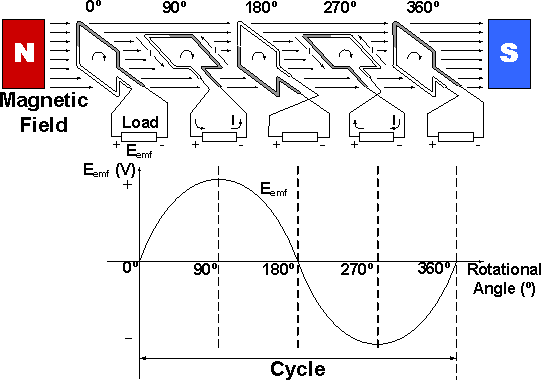
\includegraphics[scale=0.5]{rotating_coil_flux}
\end{center}

\section*{Transformers}

Transformers work by having an alternating current in a primary coil wrapped
around a solf iron core. The a.c. current induces a fluctuating magnetic field
in the iron core, which in turn induces an e.m.f in the secondary coil, since
magentic field lines are crossing the coil.

\begin{center}
	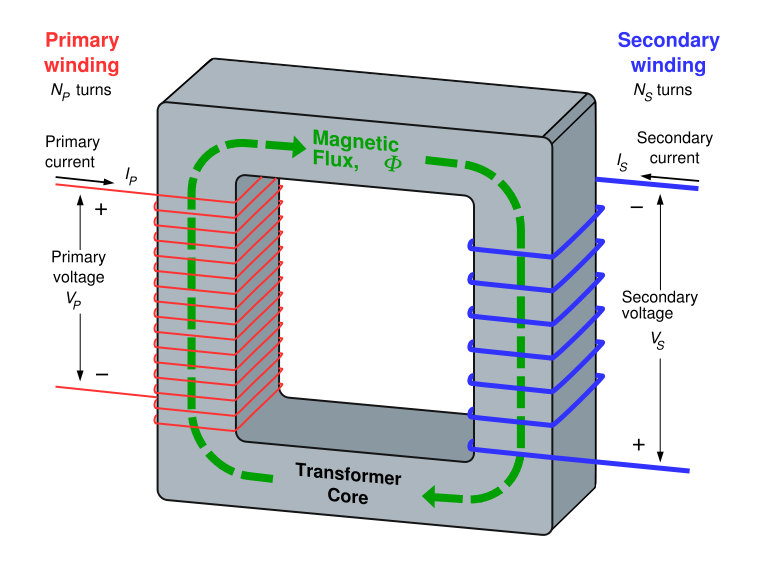
\includegraphics[scale=0.4]{transformer}
\end{center}

\subsection*{Step up and step down transformers}

The output voltage of a trnasformer depends on the ratio between the number of
coils on the primary coil and the number of coils on the secondary coil. The
equation linking the number of coils ($n$) and the voltage ($V$) is as follows:\marginpar{This is the turns ratio equation.}

\[
	\frac{V_s}{V_p} = \frac{n_s}{n_p}
\]

Where the subscripts relate to the primary ($_p$) and secondary ($_s$) coils.

Transformers that have a higher voltage across the secondary coil than the
primary coil are called step up transformers. Transformers that have a lower
voltage across the secondary coil than the primary coil are called step down
transformers.

Note that the power in the primary and secondary coil is the same (for a 100\%
efficient transformer). If the transformer is a step up transformer, it will
have a higher voltage in the secondary coil, but also a lower current. The
equation relating voltage to current is as follows:

\[
	V_pI_p = V_sI_s
\]

\end{document}